\documentclass[11pt]{article}

\usepackage{hyperref}
\usepackage{geometry}
\usepackage[T1]{fontenc}
\usepackage{natbib}
\usepackage{changepage}

% Misc packages
\usepackage{graphicx}
\usepackage{amsmath, amssymb}

% Units
\newcommand{\msun}{\textrm{M}_\odot}
\newcommand{\kpc}{\textrm{kpc}}
\newcommand{\kms}{\ensuremath{\textrm{km}~\textrm{s}^{-1}}}
\newcommand{\masyr}{\ensuremath{\textrm{mas}~\textrm{yr}^{-1}}}

% Astronomy
\newcommand{\feh}{\ensuremath{[\textrm{Fe} / \textrm{H}]}}

% page size
\geometry{
  body={6.5in, 9in},
  left=1.0in,
  top=1.0in,
  nohead,
  nofoot
}

% Title stuff
\let\apwtitle\title
\renewcommand{\apwtitle}[1]{\title{
	\vspace{-6ex}
        {\fontsize{12pt}{0em}\selectfont \textbf{#1}}
        \vspace{-6.5ex}
}}

% Change section font size and spacing
\usepackage[small,compact]{titlesec}
\titleformat{\section}{\normalfont\fontsize{12pt}{0em}\bfseries}{\thesection}{12pt}{}
\titleformat{\subsection}{\normalfont\fontsize{12pt}{0em}\bfseries}{\thesubsection}{0.5em}{}
\titleformat{\subsubsection}{\normalfont\fontsize{12pt}{2em}\bfseries}{}{0.em}{}
\titlespacing{\section}{0em}{8pt}{2pt}
\titlespacing{\subsection}{0.em}{4pt}{2pt}
\titlespacing{\subsubsection}{0em}{2pt}{2pt}

\pagenumbering{gobble}
% \setlength{\parskip}{\baselineskip}%
\setlength{\parskip}{6pt}
\setlength{\parindent}{0pt}%

\apwtitle{Deep imaging of the GD-1 stellar stream with HSC -- A. Price-Whelan et al.}
\date{}
\author{}

\setlength{\bibsep}{0pt plus 0.3ex}

\begin{document}
\maketitle

\vspace{-1em}
The clustering of dark matter on scales smaller than dwarf galaxies remains one of the most pressing unknowns in cosmology and galaxy formation (Bullock \& Boylan-Kolchin 2017).
Different dark matter theories predict different minimum mass scales for clustering: In the $\Lambda$CDM model, dark matter subhalos with negligible baryon fractions are expected to exist with masses as low as $10^{6}~\msun$ (Springel et al. 2008), while alternative models have larger cut-off masses in the dark matter power spectrum that depend on the parameters of these models (e.g., Bode et al. 2001, Hu et al. 2000).

Within the stellar halo of our Galaxy, cold stellar streams --- remnants of disrupted globular clusters (Grillmair \& Carlin 2016) --- provide a unique and powerful way to test small-scale predictions from dark matter theories.
An encounter between a stellar stream and a massive perturber alters the orderly structure of the stream by producing density variations along the stream, and can create morphological features that are not expected in simple models for stream formation (e.g., gaps, folds, and loops of debris; Yoon et al. 2011).
We recently showed that a prominent stellar stream in the Milky Way halo --- the GD-1 stream --- has several such morphological features: at least 2 gaps, with a ``spur'' of debris emanating from one gap (Price-Whelan \& Bonaca 2018).

% \section*{The GD-1 stream: a perturbed stream in the Milky Way halo}
\textbf{GD-1 perturbations as tracers of small-scale dark matter physics:}
The GD-1 stellar stream, which spans heliocentric distances $d\sim 8$--$12~\textrm{kpc}$, was discovered using photometry from the Sloan Digital Sky Survey (Grillmair \& Dionatos 2006) and has a stellar population (age $\sim 12~\textrm{Gyr}$) and width consistent with being a fully-disrupted globular cluster (Koposov et al. 2010).
% GD-1 has been used to measure the mass and shape of the large-scale mass distribution within the Galaxy (Koposov et al. 2010; Bovy et al. 2016).
% Recently, using CFHT/Megacam imaging over a $\sim 45^\circ \times 0.8^\circ$ footprint centered on the stream, de Boer at al. (2018) detected density variations along the stream and possible deviations of the main stream track that are not expected from simple models of the stream formation.
Recently, de Boer at al. (2018) detected tentative density variations along the stream using deeper CFHT/Megacam imaging.
% However, despite reaching depths of $g \sim 24$, the study only used sources brighter than $g \sim 23$ because of star--galaxy confusion.
Using astrometry from the \textit{Gaia} mission (DR2) combined with photometry from the Pan-STARRS PS1 survey, we recently mapped the stream over $\sim 100^\circ$ on the sky, producing the highest-contrast view of a cold stellar stream to date (Price-Whelan \& Bonaca 2018).
% Figure~1 (lower panel) shows a $60^\circ$ segment of the stream selected with \textit{Gaia} + PS1: black markers show the sky positions (in GD-1 coordinates) of individual stars identified as probable stream members, with some background contamination throughout the field.
Figure~1 (lower panel) shows a $60^\circ$ segment of the stream selected with \textit{Gaia} + PS1: black markers show the sky positions of probable stream members.
This relatively contamination-free view of the stream reveals two significant under-densities or ``gaps'' (e.g., Erkal \& Belokurov 2015) along the stream (indicated in Figure~1), one of which appears to have an associated spur of member stars that lies parallel to, but offset by $\sim1^\circ$ from, the main stream (Gap 1; over-density of stars located near $(\phi_1, \phi_2) \sim (-32, 1)^\circ$).

% Gaps in stellar streams with large density drops can only be formed through gravitational encounters (which can leave multiple gaps), or through the final disruption of the progenitor system (which can only explain one gap).
Gaps in stellar streams with large density drops can only be formed through gravitational encounters, or through the final disruption of the progenitor system.
\emph{The existence of two large gaps in the GD-1 stream and the presence of stream stars off of the main stream track strongly suggest that GD-1 might have encountered a dense, massive perturber, such as a dark matter subhalo.}
The origin of a gap can be inferred from the density profile of the region surrounding the gap: recently-formed subhalo gaps have characteristic ``horn''-shaped profiles (e.g., Figure~1, upper right panel).
% These density profiles encode properties of the perturber (mass and density), the geometry of the encounter (angle, impact parameter, and relative velocity), and the time of the encounter (e.g., Erkal \& Belokurov 2015).
% However, the stellar mass in these features and the density variations along streams are typically small relative to the background stellar density in our Galaxy: for a perturber mass $M \gtrsim 10^7~\msun$, and an encounter within the last orbital period, the density contrast between the horns and the stream is typically $\rho/\rho_0 \gtrsim 1.2$.
However, the induced density variations are typically small relative to the background stellar density: for a perturber mass $M \gtrsim 10^7~\msun$, and an encounter within the last orbital period, the density contrast between the horns and the stream is typically $\rho/\rho_0 \gtrsim 1.2$.
\emph{Characterizing the detailed density structure of streams therefore requires deep but wide-area photometric observations that will enable tests of dark matter theories on mass scales that are presently unreachable by any other method.}

\textbf{HSC will enable high signal-to-noise measurements of GD-1 gap profiles:}
We estimate the expected background contamination (stars and galaxies) in each proposed field using point sources (\texttt{i\_extendedness\_value == 0}) from a single HSC-SSP field at a comparable Galactic latitude to the fields proposed here.
To estimate the signal-to-noise of the stream, we use a 12 Gyr, $[\textrm{Fe}/\textrm{H}] = -1.4$ luminosity function normalized to the number of \textit{Gaia}+PS1 selected stream stars (Price-Whelan \& Bonaca 2018) in a $1.5^\circ \times 1.5^\circ$ field centered at $(\phi_1, \phi_2) = (-35, 0)^\circ$.
Figure~1 (top left) shows a simulated color-magnitude diagram (CMD) for this HSC field with simulated uncertainties for the stream stars estimated assuming a limiting $g$-band magnitude of $g \sim 25.5$.
Figure~1 (top middle) shows the signal-to-noise of the stream in a single HSC field from photometric filtering in the $g-i$ vs. $g$ CMD for 3 survey limiting magnitudes: PS1 $g \sim 22.5$, Megacam $g \sim 24$, and the proposed HSC observations $g \sim 25.5$.
To measure a 20\% density contrast, we need to reach a signal-to-noise $\textrm{S}/\textrm{N} = 30$ per field, which depends on SSP-like seeing to perform high-efficiency star-galaxy separation.
\emph{HSC is the only instrument with sufficient area to efficiently survey multiple gaps in the GD-1 stream and provide a high enough signal-to-noise to measure gap density profile variations expected from an encounter with a low-mass dark matter subhalo.}

% We propose to observe 13 HSC fields along the GD-1 stream, covering two significant gaps (Figure~1, bottom panel, red circles).

\begin{figure}[t]
\begin{center}
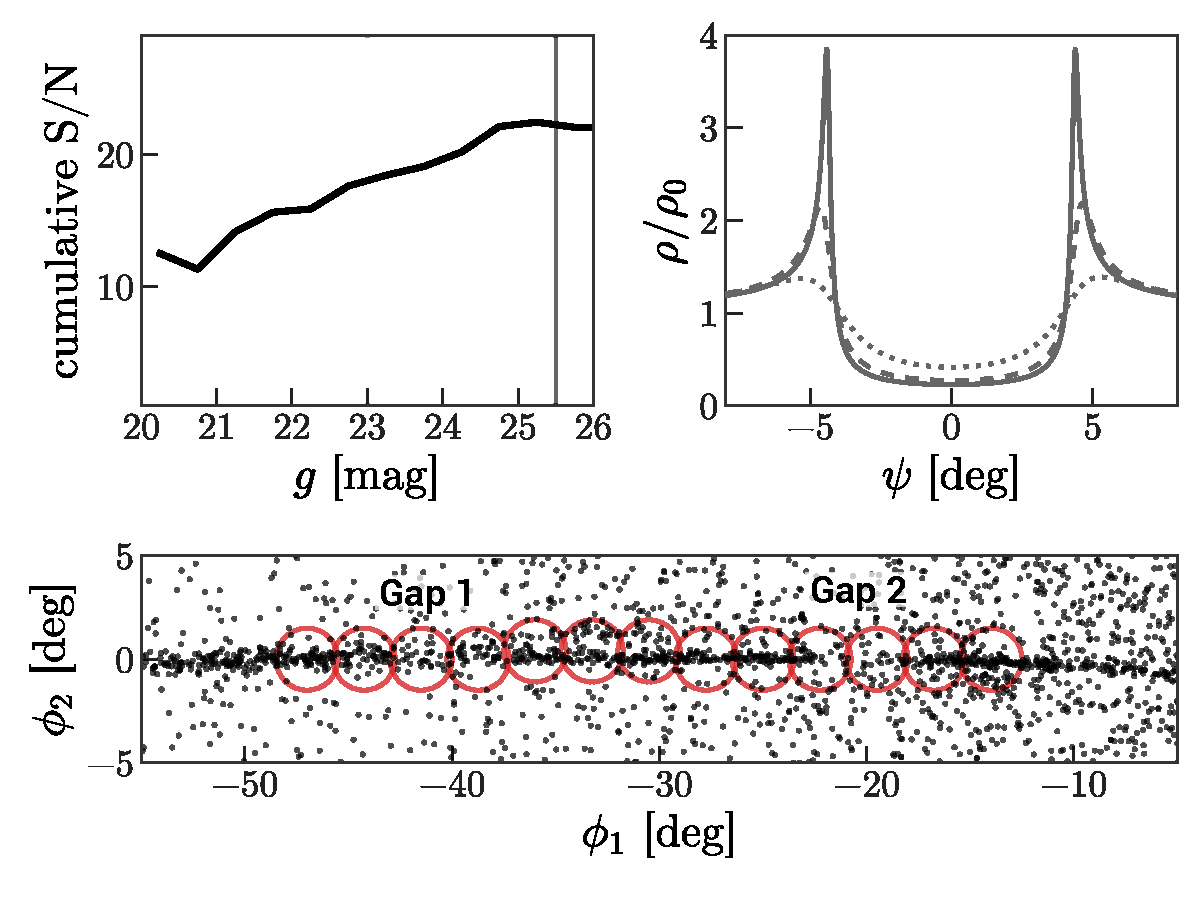
\includegraphics[width=0.9\textwidth]{figure1.pdf}
\caption{
\textbf{Top left:} Simulated GD-1 stellar population in a single HSC field super-imposed over point sources from an HSC-SSP field at the same Galactic latitude.
\textbf{Top middle:} Expected cumulative signal-to-noise, $\textrm{S}/\textrm{N} = N_{\textrm{stream}} / \sqrt{N_{\textrm{background}}}$, in a single HSC field as a function of limiting $g$ magnitude for various survey parameters.
\textbf{Top right:} Theoretical gap density profiles predicted for a low-mass ($10^7~\textrm{M}_\odot$) subhalo encounter with a GD-1 like stream at three different orientation angles.
\textbf{Bottom:} Gaia + PS1 selected GD-1 member stars (black markers) with proposed HSC pointings indicated (red circles).
}
\vspace{-1.5em}
\label{fig:}
\end{center}
\end{figure}

\textbf{References:}
Bode et al. 2001, ApJ, 556, 93 ---
Bonaca \& Hogg 2018, arXiv:1804.06854 ---
Bovy et al. 2016, arXiv:1609.01298 ---
Bullock \& Boylan-Kolchin 2017, ARAA, 55, 343 ---
Carlberg et al. 2012, ApJ, 748, 20 ---
de Boer et al. 2018, MNRAS, 477, 1893 ---
Erkal \& Belokurov 2015, MNRAS, 450, 1136 ---
Grillmair \& Dionatos 2006, ApJ, 643, L17 ---
Grillmair \& Carlin 2016, arXiv:1603.08936 ---
Hu et al. 2000, Phys. Rev. Lett., 85, 1158 ---
Koposov et al. 2010, ApJ, 712, 260 ---
Price-Whelan \& Bonaca 2018, ApJL, 863, L20 ---
Springel et al. 2008, MNRAS, 391, 1685 ---
Yoon et al. 2011, ApJ, 731, 58


\end{document}
